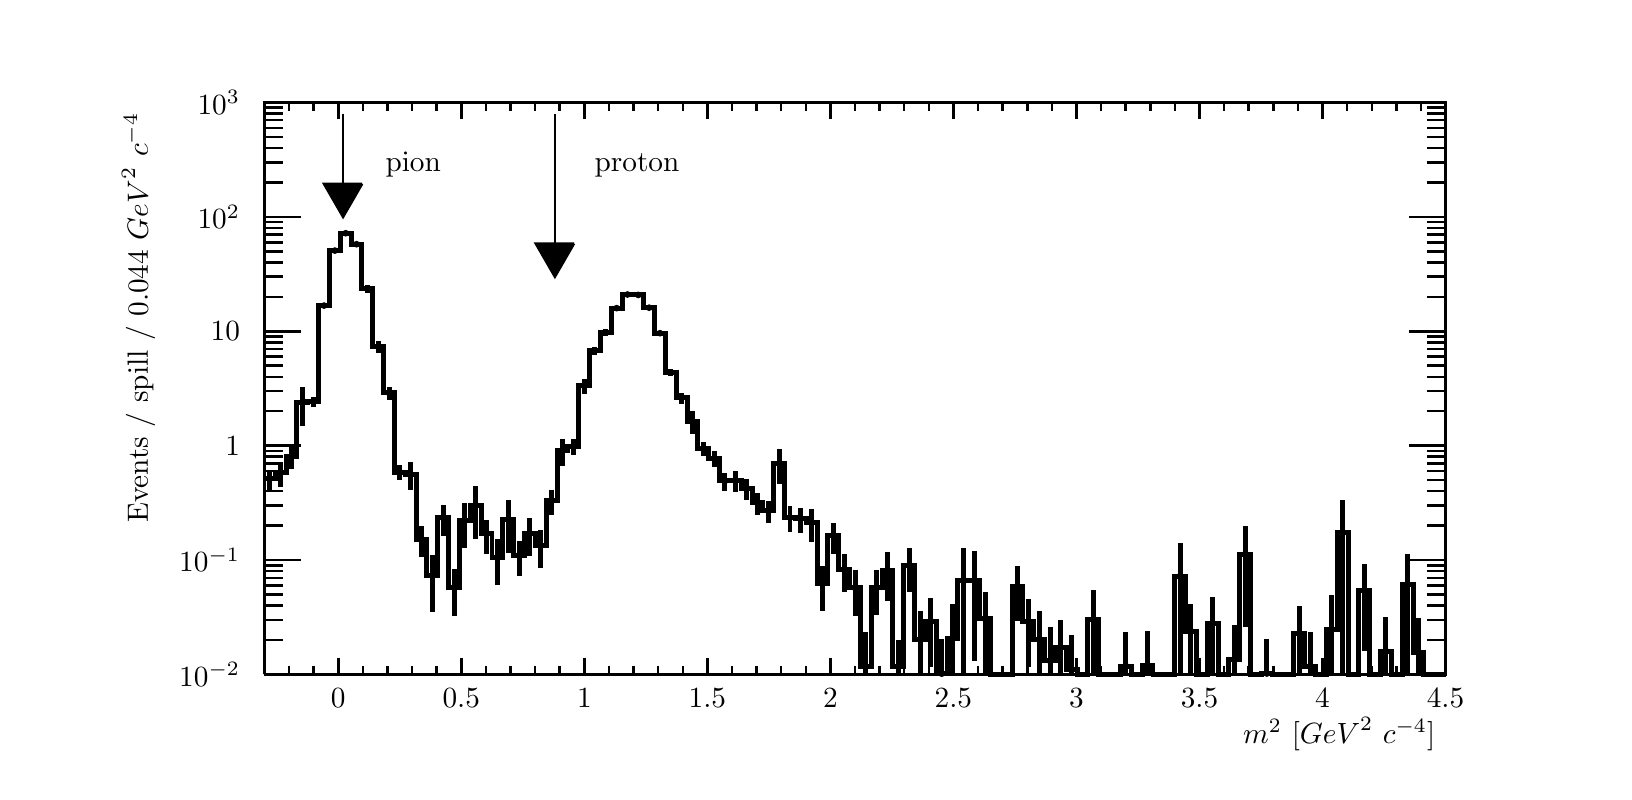
\begin{tikzpicture}
\pgfdeclareplotmark{cross} {
\pgfpathmoveto{\pgfpoint{-0.3\pgfplotmarksize}{\pgfplotmarksize}}
\pgfpathlineto{\pgfpoint{+0.3\pgfplotmarksize}{\pgfplotmarksize}}
\pgfpathlineto{\pgfpoint{+0.3\pgfplotmarksize}{0.3\pgfplotmarksize}}
\pgfpathlineto{\pgfpoint{+1\pgfplotmarksize}{0.3\pgfplotmarksize}}
\pgfpathlineto{\pgfpoint{+1\pgfplotmarksize}{-0.3\pgfplotmarksize}}
\pgfpathlineto{\pgfpoint{+0.3\pgfplotmarksize}{-0.3\pgfplotmarksize}}
\pgfpathlineto{\pgfpoint{+0.3\pgfplotmarksize}{-1.\pgfplotmarksize}}
\pgfpathlineto{\pgfpoint{-0.3\pgfplotmarksize}{-1.\pgfplotmarksize}}
\pgfpathlineto{\pgfpoint{-0.3\pgfplotmarksize}{-0.3\pgfplotmarksize}}
\pgfpathlineto{\pgfpoint{-1.\pgfplotmarksize}{-0.3\pgfplotmarksize}}
\pgfpathlineto{\pgfpoint{-1.\pgfplotmarksize}{0.3\pgfplotmarksize}}
\pgfpathlineto{\pgfpoint{-0.3\pgfplotmarksize}{0.3\pgfplotmarksize}}
\pgfpathclose
\pgfusepathqstroke
}
\pgfdeclareplotmark{cross*} {
\pgfpathmoveto{\pgfpoint{-0.3\pgfplotmarksize}{\pgfplotmarksize}}
\pgfpathlineto{\pgfpoint{+0.3\pgfplotmarksize}{\pgfplotmarksize}}
\pgfpathlineto{\pgfpoint{+0.3\pgfplotmarksize}{0.3\pgfplotmarksize}}
\pgfpathlineto{\pgfpoint{+1\pgfplotmarksize}{0.3\pgfplotmarksize}}
\pgfpathlineto{\pgfpoint{+1\pgfplotmarksize}{-0.3\pgfplotmarksize}}
\pgfpathlineto{\pgfpoint{+0.3\pgfplotmarksize}{-0.3\pgfplotmarksize}}
\pgfpathlineto{\pgfpoint{+0.3\pgfplotmarksize}{-1.\pgfplotmarksize}}
\pgfpathlineto{\pgfpoint{-0.3\pgfplotmarksize}{-1.\pgfplotmarksize}}
\pgfpathlineto{\pgfpoint{-0.3\pgfplotmarksize}{-0.3\pgfplotmarksize}}
\pgfpathlineto{\pgfpoint{-1.\pgfplotmarksize}{-0.3\pgfplotmarksize}}
\pgfpathlineto{\pgfpoint{-1.\pgfplotmarksize}{0.3\pgfplotmarksize}}
\pgfpathlineto{\pgfpoint{-0.3\pgfplotmarksize}{0.3\pgfplotmarksize}}
\pgfpathclose
\pgfusepathqfillstroke
}
\pgfdeclareplotmark{newstar} {
\pgfpathmoveto{\pgfqpoint{0pt}{\pgfplotmarksize}}
\pgfpathlineto{\pgfqpointpolar{44}{0.5\pgfplotmarksize}}
\pgfpathlineto{\pgfqpointpolar{18}{\pgfplotmarksize}}
\pgfpathlineto{\pgfqpointpolar{-20}{0.5\pgfplotmarksize}}
\pgfpathlineto{\pgfqpointpolar{-54}{\pgfplotmarksize}}
\pgfpathlineto{\pgfqpointpolar{-90}{0.5\pgfplotmarksize}}
\pgfpathlineto{\pgfqpointpolar{234}{\pgfplotmarksize}}
\pgfpathlineto{\pgfqpointpolar{198}{0.5\pgfplotmarksize}}
\pgfpathlineto{\pgfqpointpolar{162}{\pgfplotmarksize}}
\pgfpathlineto{\pgfqpointpolar{134}{0.5\pgfplotmarksize}}
\pgfpathclose
\pgfusepathqstroke
}
\pgfdeclareplotmark{newstar*} {
\pgfpathmoveto{\pgfqpoint{0pt}{\pgfplotmarksize}}
\pgfpathlineto{\pgfqpointpolar{44}{0.5\pgfplotmarksize}}
\pgfpathlineto{\pgfqpointpolar{18}{\pgfplotmarksize}}
\pgfpathlineto{\pgfqpointpolar{-20}{0.5\pgfplotmarksize}}
\pgfpathlineto{\pgfqpointpolar{-54}{\pgfplotmarksize}}
\pgfpathlineto{\pgfqpointpolar{-90}{0.5\pgfplotmarksize}}
\pgfpathlineto{\pgfqpointpolar{234}{\pgfplotmarksize}}
\pgfpathlineto{\pgfqpointpolar{198}{0.5\pgfplotmarksize}}
\pgfpathlineto{\pgfqpointpolar{162}{\pgfplotmarksize}}
\pgfpathlineto{\pgfqpointpolar{134}{0.5\pgfplotmarksize}}
\pgfpathclose
\pgfusepathqfillstroke
}
\definecolor{c}{rgb}{1,1,1};
\draw [color=c, fill=c] (0,0) rectangle (20,9.43311);
\draw [color=c, fill=c] (3,1.2263) rectangle (18,8.4898);
\definecolor{c}{rgb}{0,0,0};
\draw [c,line width=0.9] (3,1.2263) -- (3,8.4898) -- (18,8.4898) -- (18,1.2263) -- (3,1.2263);
\definecolor{c}{rgb}{1,1,1};
\draw [color=c, fill=c] (3,1.2263) rectangle (18,8.4898);
\definecolor{c}{rgb}{0,0,0};
\draw [c,line width=0.9] (3,1.2263) -- (3,8.4898) -- (18,8.4898) -- (18,1.2263) -- (3,1.2263);
\draw [c,line width=1.8] (3.06881,3.56872) -- (3.06881,3.71136);
\draw [c,line width=1.8] (3.06881,3.71136) -- (3.06881,3.82762);
\foreach \P in {(3.06881,3.71136)}{\draw[mark options={color=c,fill=c},mark size=2.402402pt,mark=*,mark size=1pt] plot coordinates {\P};}
\draw [c,line width=1.8] (3.20642,3.60405) -- (3.20642,3.78774);
\draw [c,line width=1.8] (3.20642,3.78774) -- (3.20642,3.92983);
\foreach \P in {(3.20642,3.78774)}{\draw[mark options={color=c,fill=c},mark size=2.402402pt,mark=*,mark size=1pt] plot coordinates {\P};}
\draw [c,line width=1.8] (3.34404,3.83272) -- (3.34404,3.99102);
\draw [c,line width=1.8] (3.34404,3.99102) -- (3.34404,4.11746);
\foreach \P in {(3.34404,3.99102)}{\draw[mark options={color=c,fill=c},mark size=2.402402pt,mark=*,mark size=1pt] plot coordinates {\P};}
\draw [c,line width=1.8] (3.48165,4.37763) -- (3.48165,4.6782);
\draw [c,line width=1.8] (3.48165,4.6782) -- (3.48165,4.88094);
\foreach \P in {(3.48165,4.6782)}{\draw[mark options={color=c,fill=c},mark size=2.402402pt,mark=*,mark size=1pt] plot coordinates {\P};}
\draw [c,line width=1.8] (3.61927,4.62245) -- (3.61927,4.6917);
\draw [c,line width=1.8] (3.61927,4.6917) -- (3.61927,4.7541);
\foreach \P in {(3.61927,4.6917)}{\draw[mark options={color=c,fill=c},mark size=2.402402pt,mark=*,mark size=1pt] plot coordinates {\P};}
\draw [c,line width=1.8] (3.75688,5.88089) -- (3.75688,5.91059);
\draw [c,line width=1.8] (3.75688,5.91059) -- (3.75688,5.93895);
\foreach \P in {(3.75688,5.91059)}{\draw[mark options={color=c,fill=c},mark size=2.402402pt,mark=*,mark size=1pt] plot coordinates {\P};}
\draw [c,line width=1.8] (3.8945,6.58821) -- (3.8945,6.609);
\draw [c,line width=1.8] (3.8945,6.609) -- (3.8945,6.62913);
\foreach \P in {(3.8945,6.609)}{\draw[mark options={color=c,fill=c},mark size=2.402402pt,mark=*,mark size=1pt] plot coordinates {\P};}
\draw [c,line width=1.8] (4.03211,6.80875) -- (4.03211,6.8294);
\draw [c,line width=1.8] (4.03211,6.8294) -- (4.03211,6.8494);
\foreach \P in {(4.03211,6.8294)}{\draw[mark options={color=c,fill=c},mark size=2.402402pt,mark=*,mark size=1pt] plot coordinates {\P};}
\draw [c,line width=1.8] (4.16972,6.66216) -- (4.16972,6.68997);
\draw [c,line width=1.8] (4.16972,6.68997) -- (4.16972,6.7166);
\foreach \P in {(4.16972,6.68997)}{\draw[mark options={color=c,fill=c},mark size=2.402402pt,mark=*,mark size=1pt] plot coordinates {\P};}
\draw [c,line width=1.8] (4.30734,6.07616) -- (4.30734,6.12807);
\draw [c,line width=1.8] (4.30734,6.12807) -- (4.30734,6.17604);
\foreach \P in {(4.30734,6.12807)}{\draw[mark options={color=c,fill=c},mark size=2.402402pt,mark=*,mark size=1pt] plot coordinates {\P};}
\draw [c,line width=1.8] (4.44495,5.31081) -- (4.44495,5.39135);
\draw [c,line width=1.8] (4.44495,5.39135) -- (4.44495,5.46277);
\foreach \P in {(4.44495,5.39135)}{\draw[mark options={color=c,fill=c},mark size=2.402402pt,mark=*,mark size=1pt] plot coordinates {\P};}
\draw [c,line width=1.8] (4.58257,4.71441) -- (4.58257,4.80088);
\draw [c,line width=1.8] (4.58257,4.80088) -- (4.58257,4.87692);
\foreach \P in {(4.58257,4.80088)}{\draw[mark options={color=c,fill=c},mark size=2.402402pt,mark=*,mark size=1pt] plot coordinates {\P};}
\draw [c,line width=1.8] (4.72018,3.69222) -- (4.72018,3.794);
\draw [c,line width=1.8] (4.72018,3.794) -- (4.72018,3.88161);
\foreach \P in {(4.72018,3.794)}{\draw[mark options={color=c,fill=c},mark size=2.402402pt,mark=*,mark size=1pt] plot coordinates {\P};}
\draw [c,line width=1.8] (4.8578,3.56322) -- (4.8578,3.7652);
\draw [c,line width=1.8] (4.8578,3.7652) -- (4.8578,3.91796);
\foreach \P in {(4.8578,3.7652)}{\draw[mark options={color=c,fill=c},mark size=2.402402pt,mark=*,mark size=1pt] plot coordinates {\P};}
\draw [c,line width=1.8] (4.99541,2.72369) -- (4.99541,2.944);
\draw [c,line width=1.8] (4.99541,2.944) -- (4.99541,3.10698);
\foreach \P in {(4.99541,2.944)}{\draw[mark options={color=c,fill=c},mark size=2.402402pt,mark=*,mark size=1pt] plot coordinates {\P};}
\draw [c,line width=1.8] (5.13303,2.02126) -- (5.13303,2.48397);
\draw [c,line width=1.8] (5.13303,2.48397) -- (5.13303,2.74802);
\foreach \P in {(5.13303,2.48397)}{\draw[mark options={color=c,fill=c},mark size=2.402402pt,mark=*,mark size=1pt] plot coordinates {\P};}
\draw [c,line width=1.8] (5.27064,2.98961) -- (5.27064,3.21415);
\draw [c,line width=1.8] (5.27064,3.21415) -- (5.27064,3.37941);
\foreach \P in {(5.27064,3.21415)}{\draw[mark options={color=c,fill=c},mark size=2.402402pt,mark=*,mark size=1pt] plot coordinates {\P};}
\draw [c,line width=1.8] (5.40826,1.96462) -- (5.40826,2.33111);
\draw [c,line width=1.8] (5.40826,2.33111) -- (5.40826,2.56143);
\foreach \P in {(5.40826,2.33111)}{\draw[mark options={color=c,fill=c},mark size=2.402402pt,mark=*,mark size=1pt] plot coordinates {\P};}
\draw [c,line width=1.8] (5.54587,2.82628) -- (5.54587,3.17889);
\draw [c,line width=1.8] (5.54587,3.17889) -- (5.54587,3.40373);
\foreach \P in {(5.54587,3.17889)}{\draw[mark options={color=c,fill=c},mark size=2.402402pt,mark=*,mark size=1pt] plot coordinates {\P};}
\draw [c,line width=1.8] (5.68349,2.95178) -- (5.68349,3.37453);
\draw [c,line width=1.8] (5.68349,3.37453) -- (5.68349,3.62542);
\foreach \P in {(5.68349,3.37453)}{\draw[mark options={color=c,fill=c},mark size=2.402402pt,mark=*,mark size=1pt] plot coordinates {\P};}
\draw [c,line width=1.8] (5.8211,2.75545) -- (5.8211,3.01109);
\draw [c,line width=1.8] (5.8211,3.01109) -- (5.8211,3.19251);
\foreach \P in {(5.8211,3.01109)}{\draw[mark options={color=c,fill=c},mark size=2.402402pt,mark=*,mark size=1pt] plot coordinates {\P};}
\draw [c,line width=1.8] (5.95872,2.3592) -- (5.95872,2.71711);
\draw [c,line width=1.8] (5.95872,2.71711) -- (5.95872,2.94407);
\foreach \P in {(5.95872,2.71711)}{\draw[mark options={color=c,fill=c},mark size=2.402402pt,mark=*,mark size=1pt] plot coordinates {\P};}
\draw [c,line width=1.8] (6.09633,2.76628) -- (6.09633,3.19469);
\draw [c,line width=1.8] (6.09633,3.19469) -- (6.09633,3.4475);
\foreach \P in {(6.09633,3.19469)}{\draw[mark options={color=c,fill=c},mark size=2.402402pt,mark=*,mark size=1pt] plot coordinates {\P};}
\draw [c,line width=1.8] (6.23394,2.47429) -- (6.23394,2.73953);
\draw [c,line width=1.8] (6.23394,2.73953) -- (6.23394,2.92569);
\foreach \P in {(6.23394,2.73953)}{\draw[mark options={color=c,fill=c},mark size=2.402402pt,mark=*,mark size=1pt] plot coordinates {\P};}
\draw [c,line width=1.8] (6.37156,2.73579) -- (6.37156,3.01506);
\draw [c,line width=1.8] (6.37156,3.01506) -- (6.37156,3.20796);
\foreach \P in {(6.37156,3.01506)}{\draw[mark options={color=c,fill=c},mark size=2.402402pt,mark=*,mark size=1pt] plot coordinates {\P};}
\draw [c,line width=1.8] (6.50917,2.57445) -- (6.50917,2.86253);
\draw [c,line width=1.8] (6.50917,2.86253) -- (6.50917,3.05956);
\foreach \P in {(6.50917,2.86253)}{\draw[mark options={color=c,fill=c},mark size=2.402402pt,mark=*,mark size=1pt] plot coordinates {\P};}
\draw [c,line width=1.8] (6.64679,3.25685) -- (6.64679,3.42962);
\draw [c,line width=1.8] (6.64679,3.42962) -- (6.64679,3.56511);
\foreach \P in {(6.64679,3.42962)}{\draw[mark options={color=c,fill=c},mark size=2.402402pt,mark=*,mark size=1pt] plot coordinates {\P};}
\draw [c,line width=1.8] (6.7844,3.87258) -- (6.7844,4.06998);
\draw [c,line width=1.8] (6.7844,4.06998) -- (6.7844,4.22011);
\foreach \P in {(6.7844,4.06998)}{\draw[mark options={color=c,fill=c},mark size=2.402402pt,mark=*,mark size=1pt] plot coordinates {\P};}
\draw [c,line width=1.8] (6.92202,4.0118) -- (6.92202,4.12585);
\draw [c,line width=1.8] (6.92202,4.12585) -- (6.92202,4.22241);
\foreach \P in {(6.92202,4.12585)}{\draw[mark options={color=c,fill=c},mark size=2.402402pt,mark=*,mark size=1pt] plot coordinates {\P};}
\draw [c,line width=1.8] (7.05963,4.78915) -- (7.05963,4.89028);
\draw [c,line width=1.8] (7.05963,4.89028) -- (7.05963,4.97742);
\foreach \P in {(7.05963,4.89028)}{\draw[mark options={color=c,fill=c},mark size=2.402402pt,mark=*,mark size=1pt] plot coordinates {\P};}
\draw [c,line width=1.8] (7.19725,5.28396) -- (7.19725,5.33785);
\draw [c,line width=1.8] (7.19725,5.33785) -- (7.19725,5.3875);
\foreach \P in {(7.19725,5.33785)}{\draw[mark options={color=c,fill=c},mark size=2.402402pt,mark=*,mark size=1pt] plot coordinates {\P};}
\draw [c,line width=1.8] (7.33486,5.52386) -- (7.33486,5.57101);
\draw [c,line width=1.8] (7.33486,5.57101) -- (7.33486,5.61488);
\foreach \P in {(7.33486,5.57101)}{\draw[mark options={color=c,fill=c},mark size=2.402402pt,mark=*,mark size=1pt] plot coordinates {\P};}
\draw [c,line width=1.8] (7.47248,5.84918) -- (7.47248,5.87775);
\draw [c,line width=1.8] (7.47248,5.87775) -- (7.47248,5.90507);
\foreach \P in {(7.47248,5.87775)}{\draw[mark options={color=c,fill=c},mark size=2.402402pt,mark=*,mark size=1pt] plot coordinates {\P};}
\draw [c,line width=1.8] (7.61009,6.02421) -- (7.61009,6.05102);
\draw [c,line width=1.8] (7.61009,6.05102) -- (7.61009,6.07674);
\foreach \P in {(7.61009,6.05102)}{\draw[mark options={color=c,fill=c},mark size=2.402402pt,mark=*,mark size=1pt] plot coordinates {\P};}
\draw [c,line width=1.8] (7.74771,6.02286) -- (7.74771,6.046);
\draw [c,line width=1.8] (7.74771,6.046) -- (7.74771,6.06832);
\foreach \P in {(7.74771,6.046)}{\draw[mark options={color=c,fill=c},mark size=2.402402pt,mark=*,mark size=1pt] plot coordinates {\P};}
\draw [c,line width=1.8] (7.88532,5.85613) -- (7.88532,5.8838);
\draw [c,line width=1.8] (7.88532,5.8838) -- (7.88532,5.91031);
\foreach \P in {(7.88532,5.8838)}{\draw[mark options={color=c,fill=c},mark size=2.402402pt,mark=*,mark size=1pt] plot coordinates {\P};}
\draw [c,line width=1.8] (8.02294,5.52535) -- (8.02294,5.56009);
\draw [c,line width=1.8] (8.02294,5.56009) -- (8.02294,5.59301);
\foreach \P in {(8.02294,5.56009)}{\draw[mark options={color=c,fill=c},mark size=2.402402pt,mark=*,mark size=1pt] plot coordinates {\P};}
\draw [c,line width=1.8] (8.16055,5.01206) -- (8.16055,5.0609);
\draw [c,line width=1.8] (8.16055,5.0609) -- (8.16055,5.10624);
\foreach \P in {(8.16055,5.0609)}{\draw[mark options={color=c,fill=c},mark size=2.402402pt,mark=*,mark size=1pt] plot coordinates {\P};}
\draw [c,line width=1.8] (8.29817,4.66691) -- (8.29817,4.73945);
\draw [c,line width=1.8] (8.29817,4.73945) -- (8.29817,4.80449);
\foreach \P in {(8.29817,4.73945)}{\draw[mark options={color=c,fill=c},mark size=2.402402pt,mark=*,mark size=1pt] plot coordinates {\P};}
\draw [c,line width=1.8] (8.43578,4.28359) -- (8.43578,4.44033);
\draw [c,line width=1.8] (8.43578,4.44033) -- (8.43578,4.56577);
\foreach \P in {(8.43578,4.44033)}{\draw[mark options={color=c,fill=c},mark size=2.402402pt,mark=*,mark size=1pt] plot coordinates {\P};}
\draw [c,line width=1.8] (8.57339,3.99655) -- (8.57339,4.09149);
\draw [c,line width=1.8] (8.57339,4.09149) -- (8.57339,4.174);
\foreach \P in {(8.57339,4.09149)}{\draw[mark options={color=c,fill=c},mark size=2.402402pt,mark=*,mark size=1pt] plot coordinates {\P};}
\draw [c,line width=1.8] (8.71101,3.85907) -- (8.71101,3.96865);
\draw [c,line width=1.8] (8.71101,3.96865) -- (8.71101,4.06199);
\foreach \P in {(8.71101,3.96865)}{\draw[mark options={color=c,fill=c},mark size=2.402402pt,mark=*,mark size=1pt] plot coordinates {\P};}
\draw [c,line width=1.8] (8.84862,3.56063) -- (8.84862,3.68393);
\draw [c,line width=1.8] (8.84862,3.68393) -- (8.84862,3.78703);
\foreach \P in {(8.84862,3.68393)}{\draw[mark options={color=c,fill=c},mark size=2.402402pt,mark=*,mark size=1pt] plot coordinates {\P};}
\draw [c,line width=1.8] (8.98624,3.54614) -- (8.98624,3.69032);
\draw [c,line width=1.8] (8.98624,3.69032) -- (8.98624,3.8076);
\foreach \P in {(8.98624,3.69032)}{\draw[mark options={color=c,fill=c},mark size=2.402402pt,mark=*,mark size=1pt] plot coordinates {\P};}
\draw [c,line width=1.8] (9.12385,3.44504) -- (9.12385,3.58819);
\draw [c,line width=1.8] (9.12385,3.58819) -- (9.12385,3.70479);
\foreach \P in {(9.12385,3.58819)}{\draw[mark options={color=c,fill=c},mark size=2.402402pt,mark=*,mark size=1pt] plot coordinates {\P};}
\draw [c,line width=1.8] (9.26147,3.2554) -- (9.26147,3.41055);
\draw [c,line width=1.8] (9.26147,3.41055) -- (9.26147,3.53499);
\foreach \P in {(9.26147,3.41055)}{\draw[mark options={color=c,fill=c},mark size=2.402402pt,mark=*,mark size=1pt] plot coordinates {\P};}
\draw [c,line width=1.8] (9.39908,3.14598) -- (9.39908,3.30399);
\draw [c,line width=1.8] (9.39908,3.30399) -- (9.39908,3.43025);
\foreach \P in {(9.39908,3.30399)}{\draw[mark options={color=c,fill=c},mark size=2.402402pt,mark=*,mark size=1pt] plot coordinates {\P};}
\draw [c,line width=1.8] (9.5367,3.64807) -- (9.5367,3.90256);
\draw [c,line width=1.8] (9.5367,3.90256) -- (9.5367,4.0834);
\foreach \P in {(9.5367,3.90256)}{\draw[mark options={color=c,fill=c},mark size=2.402402pt,mark=*,mark size=1pt] plot coordinates {\P};}
\draw [c,line width=1.8] (9.67431,3.03567) -- (9.67431,3.21987);
\draw [c,line width=1.8] (9.67431,3.21987) -- (9.67431,3.36227);
\foreach \P in {(9.67431,3.21987)}{\draw[mark options={color=c,fill=c},mark size=2.402402pt,mark=*,mark size=1pt] plot coordinates {\P};}
\draw [c,line width=1.8] (9.81193,3.02432) -- (9.81193,3.2043);
\draw [c,line width=1.8] (9.81193,3.2043) -- (9.81193,3.34417);
\foreach \P in {(9.81193,3.2043)}{\draw[mark options={color=c,fill=c},mark size=2.402402pt,mark=*,mark size=1pt] plot coordinates {\P};}
\draw [c,line width=1.8] (9.94954,2.90575) -- (9.94954,3.15507);
\draw [c,line width=1.8] (9.94954,3.15507) -- (9.94954,3.33329);
\foreach \P in {(9.94954,3.15507)}{\draw[mark options={color=c,fill=c},mark size=2.402402pt,mark=*,mark size=1pt] plot coordinates {\P};}
\draw [c,line width=1.8] (10.0872,2.03789) -- (10.0872,2.38235);
\draw [c,line width=1.8] (10.0872,2.38235) -- (10.0872,2.6039);
\foreach \P in {(10.0872,2.38235)}{\draw[mark options={color=c,fill=c},mark size=2.402402pt,mark=*,mark size=1pt] plot coordinates {\P};}
\draw [c,line width=1.8] (10.2248,2.75862) -- (10.2248,2.98477);
\draw [c,line width=1.8] (10.2248,2.98477) -- (10.2248,3.1509);
\foreach \P in {(10.2248,2.98477)}{\draw[mark options={color=c,fill=c},mark size=2.402402pt,mark=*,mark size=1pt] plot coordinates {\P};}
\draw [c,line width=1.8] (10.3624,2.27162) -- (10.3624,2.5586);
\draw [c,line width=1.8] (10.3624,2.5586) -- (10.3624,2.75512);
\foreach \P in {(10.3624,2.5586)}{\draw[mark options={color=c,fill=c},mark size=2.402402pt,mark=*,mark size=1pt] plot coordinates {\P};}
\draw [c,line width=1.8] (10.5,1.96858) -- (10.5,2.32496);
\draw [c,line width=1.8] (10.5,2.32496) -- (10.5,2.55131);
\foreach \P in {(10.5,2.32496)}{\draw[mark options={color=c,fill=c},mark size=2.402402pt,mark=*,mark size=1pt] plot coordinates {\P};}
\draw [c,line width=1.8] (10.6376,1.2263) -- (10.6376,1.3277);
\draw [c,line width=1.8] (10.6376,1.3277) -- (10.6376,1.76537);
\foreach \P in {(10.6376,1.3277)}{\draw[mark options={color=c,fill=c},mark size=2.402402pt,mark=*,mark size=1pt] plot coordinates {\P};}
\draw [c,line width=1.8] (10.7752,1.98377) -- (10.7752,2.32996);
\draw [c,line width=1.8] (10.7752,2.32996) -- (10.7752,2.55221);
\foreach \P in {(10.7752,2.32996)}{\draw[mark options={color=c,fill=c},mark size=2.402402pt,mark=*,mark size=1pt] plot coordinates {\P};}
\draw [c,line width=1.8] (10.9128,2.15956) -- (10.9128,2.54358);
\draw [c,line width=1.8] (10.9128,2.54358) -- (10.9128,2.78057);
\foreach \P in {(10.9128,2.54358)}{\draw[mark options={color=c,fill=c},mark size=2.402402pt,mark=*,mark size=1pt] plot coordinates {\P};}
\draw [c,line width=1.8] (11.0505,1.2263) -- (11.0505,1.32725);
\draw [c,line width=1.8] (11.0505,1.32725) -- (11.0505,1.6654);
\foreach \P in {(11.0505,1.32725)}{\draw[mark options={color=c,fill=c},mark size=2.402402pt,mark=*,mark size=1pt] plot coordinates {\P};}
\draw [c,line width=1.8] (11.1881,2.27742) -- (11.1881,2.61114);
\draw [c,line width=1.8] (11.1881,2.61114) -- (11.1881,2.82825);
\foreach \P in {(11.1881,2.61114)}{\draw[mark options={color=c,fill=c},mark size=2.402402pt,mark=*,mark size=1pt] plot coordinates {\P};}
\draw [c,line width=1.8] (11.3257,1.2263) -- (11.3257,1.67205);
\draw [c,line width=1.8] (11.3257,1.67205) -- (11.3257,2.03101);
\foreach \P in {(11.3257,1.67205)}{\draw[mark options={color=c,fill=c},mark size=2.402402pt,mark=*,mark size=1pt] plot coordinates {\P};}
\draw [c,line width=1.8] (11.4633,1.32341) -- (11.4633,1.90285);
\draw [c,line width=1.8] (11.4633,1.90285) -- (11.4633,2.19972);
\foreach \P in {(11.4633,1.90285)}{\draw[mark options={color=c,fill=c},mark size=2.402402pt,mark=*,mark size=1pt] plot coordinates {\P};}
\draw [c,line width=1.8] (11.6009,1.2263) -- (11.6009,1.23591);
\draw [c,line width=1.8] (11.6009,1.23591) -- (11.6009,1.67363);
\foreach \P in {(11.6009,1.23591)}{\draw[mark options={color=c,fill=c},mark size=2.402402pt,mark=*,mark size=1pt] plot coordinates {\P};}
\draw [c,line width=1.8] (11.7385,1.2263) -- (11.7385,1.68607);
\draw [c,line width=1.8] (11.7385,1.68607) -- (11.7385,2.12389);
\foreach \P in {(11.7385,1.68607)}{\draw[mark options={color=c,fill=c},mark size=2.402402pt,mark=*,mark size=1pt] plot coordinates {\P};}
\draw [c,line width=1.8] (11.8761,1.2263) -- (11.8761,2.4233);
\draw [c,line width=1.8] (11.8761,2.4233) -- (11.8761,2.834);
\foreach \P in {(11.8761,2.4233)}{\draw[mark options={color=c,fill=c},mark size=2.402402pt,mark=*,mark size=1pt] plot coordinates {\P};}
\draw [c,line width=1.8] (12.0138,1.39728) -- (12.0138,2.4205);
\draw [c,line width=1.8] (12.0138,2.4205) -- (12.0138,2.79219);
\foreach \P in {(12.0138,2.4205)}{\draw[mark options={color=c,fill=c},mark size=2.402402pt,mark=*,mark size=1pt] plot coordinates {\P};}
\draw [c,line width=1.8] (12.1514,1.2263) -- (12.1514,1.93107);
\draw [c,line width=1.8] (12.1514,1.93107) -- (12.1514,2.27464);
\foreach \P in {(12.1514,1.93107)}{\draw[mark options={color=c,fill=c},mark size=2.402402pt,mark=*,mark size=1pt] plot coordinates {\P};}
\draw [c,line width=1.8] (12.5642,1.90555) -- (12.5642,2.34491);
\draw [c,line width=1.8] (12.5642,2.34491) -- (12.5642,2.60141);
\foreach \P in {(12.5642,2.34491)}{\draw[mark options={color=c,fill=c},mark size=2.402402pt,mark=*,mark size=1pt] plot coordinates {\P};}
\draw [c,line width=1.8] (12.7018,1.31527) -- (12.7018,1.89266);
\draw [c,line width=1.8] (12.7018,1.89266) -- (12.7018,2.18901);
\foreach \P in {(12.7018,1.89266)}{\draw[mark options={color=c,fill=c},mark size=2.402402pt,mark=*,mark size=1pt] plot coordinates {\P};}
\draw [c,line width=1.8] (12.8394,1.2263) -- (12.8394,1.6727);
\draw [c,line width=1.8] (12.8394,1.6727) -- (12.8394,2.03107);
\foreach \P in {(12.8394,1.6727)}{\draw[mark options={color=c,fill=c},mark size=2.402402pt,mark=*,mark size=1pt] plot coordinates {\P};}
\draw [c,line width=1.8] (12.9771,1.2263) -- (12.9771,1.39712);
\draw [c,line width=1.8] (12.9771,1.39712) -- (12.9771,1.83482);
\foreach \P in {(12.9771,1.39712)}{\draw[mark options={color=c,fill=c},mark size=2.402402pt,mark=*,mark size=1pt] plot coordinates {\P};}
\draw [c,line width=1.8] (13.1147,1.2263) -- (13.1147,1.5685);
\draw [c,line width=1.8] (13.1147,1.5685) -- (13.1147,1.9191);
\foreach \P in {(13.1147,1.5685)}{\draw[mark options={color=c,fill=c},mark size=2.402402pt,mark=*,mark size=1pt] plot coordinates {\P};}
\draw [c,line width=1.8] (13.2523,1.2263) -- (13.2523,1.2852);
\draw [c,line width=1.8] (13.2523,1.2852) -- (13.2523,1.72288);
\foreach \P in {(13.2523,1.2852)}{\draw[mark options={color=c,fill=c},mark size=2.402402pt,mark=*,mark size=1pt] plot coordinates {\P};}
\draw [c,line width=1.8] (13.5275,1.2263) -- (13.5275,1.92356);
\draw [c,line width=1.8] (13.5275,1.92356) -- (13.5275,2.30434);
\foreach \P in {(13.5275,1.92356)}{\draw[mark options={color=c,fill=c},mark size=2.402402pt,mark=*,mark size=1pt] plot coordinates {\P};}
\draw [c,line width=1.8] (13.9404,1.2263) -- (13.9404,1.33199);
\draw [c,line width=1.8] (13.9404,1.33199) -- (13.9404,1.76967);
\foreach \P in {(13.9404,1.33199)}{\draw[mark options={color=c,fill=c},mark size=2.402402pt,mark=*,mark size=1pt] plot coordinates {\P};}
\draw [c,line width=1.8] (14.2156,1.2263) -- (14.2156,1.34151);
\draw [c,line width=1.8] (14.2156,1.34151) -- (14.2156,1.77924);
\foreach \P in {(14.2156,1.34151)}{\draw[mark options={color=c,fill=c},mark size=2.402402pt,mark=*,mark size=1pt] plot coordinates {\P};}
\draw [c,line width=1.8] (14.6284,1.2263) -- (14.6284,2.47584);
\draw [c,line width=1.8] (14.6284,2.47584) -- (14.6284,2.88914);
\foreach \P in {(14.6284,2.47584)}{\draw[mark options={color=c,fill=c},mark size=2.402402pt,mark=*,mark size=1pt] plot coordinates {\P};}
\draw [c,line width=1.8] (14.7661,1.2263) -- (14.7661,1.77723);
\draw [c,line width=1.8] (14.7661,1.77723) -- (14.7661,2.11494);
\foreach \P in {(14.7661,1.77723)}{\draw[mark options={color=c,fill=c},mark size=2.402402pt,mark=*,mark size=1pt] plot coordinates {\P};}
\draw [c,line width=1.8] (15.0413,1.2263) -- (15.0413,1.86949);
\draw [c,line width=1.8] (15.0413,1.86949) -- (15.0413,2.21436);
\foreach \P in {(15.0413,1.86949)}{\draw[mark options={color=c,fill=c},mark size=2.402402pt,mark=*,mark size=1pt] plot coordinates {\P};}
\draw [c,line width=1.8] (15.3165,1.2263) -- (15.3165,1.41421);
\draw [c,line width=1.8] (15.3165,1.41421) -- (15.3165,1.85179);
\foreach \P in {(15.3165,1.41421)}{\draw[mark options={color=c,fill=c},mark size=2.402402pt,mark=*,mark size=1pt] plot coordinates {\P};}
\draw [c,line width=1.8] (15.4541,1.82819) -- (15.4541,2.75279);
\draw [c,line width=1.8] (15.4541,2.75279) -- (15.4541,3.11268);
\foreach \P in {(15.4541,2.75279)}{\draw[mark options={color=c,fill=c},mark size=2.402402pt,mark=*,mark size=1pt] plot coordinates {\P};}
\draw [c,line width=1.8] (15.7294,1.2263) -- (15.7294,1.23755);
\draw [c,line width=1.8] (15.7294,1.23755) -- (15.7294,1.67527);
\foreach \P in {(15.7294,1.23755)}{\draw[mark options={color=c,fill=c},mark size=2.402402pt,mark=*,mark size=1pt] plot coordinates {\P};}
\draw [c,line width=1.8] (16.1422,1.2263) -- (16.1422,1.75095);
\draw [c,line width=1.8] (16.1422,1.75095) -- (16.1422,2.09382);
\foreach \P in {(16.1422,1.75095)}{\draw[mark options={color=c,fill=c},mark size=2.402402pt,mark=*,mark size=1pt] plot coordinates {\P};}
\draw [c,line width=1.8] (16.2798,1.2263) -- (16.2798,1.33171);
\draw [c,line width=1.8] (16.2798,1.33171) -- (16.2798,1.76939);
\foreach \P in {(16.2798,1.33171)}{\draw[mark options={color=c,fill=c},mark size=2.402402pt,mark=*,mark size=1pt] plot coordinates {\P};}
\draw [c,line width=1.8] (16.555,1.2263) -- (16.555,1.7949);
\draw [c,line width=1.8] (16.555,1.7949) -- (16.555,2.23253);
\foreach \P in {(16.555,1.7949)}{\draw[mark options={color=c,fill=c},mark size=2.402402pt,mark=*,mark size=1pt] plot coordinates {\P};}
\draw [c,line width=1.8] (16.6927,1.2263) -- (16.6927,3.02411);
\draw [c,line width=1.8] (16.6927,3.02411) -- (16.6927,3.44421);
\foreach \P in {(16.6927,3.02411)}{\draw[mark options={color=c,fill=c},mark size=2.402402pt,mark=*,mark size=1pt] plot coordinates {\P};}
\draw [c,line width=1.8] (16.9679,1.52976) -- (16.9679,2.28801);
\draw [c,line width=1.8] (16.9679,2.28801) -- (16.9679,2.62255);
\foreach \P in {(16.9679,2.28801)}{\draw[mark options={color=c,fill=c},mark size=2.402402pt,mark=*,mark size=1pt] plot coordinates {\P};}
\draw [c,line width=1.8] (17.2431,1.2263) -- (17.2431,1.52343);
\draw [c,line width=1.8] (17.2431,1.52343) -- (17.2431,1.96114);
\foreach \P in {(17.2431,1.52343)}{\draw[mark options={color=c,fill=c},mark size=2.402402pt,mark=*,mark size=1pt] plot coordinates {\P};}
\draw [c,line width=1.8] (17.5183,1.24079) -- (17.5183,2.37168);
\draw [c,line width=1.8] (17.5183,2.37168) -- (17.5183,2.75413);
\foreach \P in {(17.5183,2.37168)}{\draw[mark options={color=c,fill=c},mark size=2.402402pt,mark=*,mark size=1pt] plot coordinates {\P};}
\draw [c,line width=1.8] (17.656,1.2263) -- (17.656,1.50107);
\draw [c,line width=1.8] (17.656,1.50107) -- (17.656,1.93861);
\foreach \P in {(17.656,1.50107)}{\draw[mark options={color=c,fill=c},mark size=2.402402pt,mark=*,mark size=1pt] plot coordinates {\P};}
\draw [c,line width=1.8] (3,3.71136) -- (3.13761,3.71136) -- (3.13761,3.78774) -- (3.27523,3.78774) -- (3.27523,3.99102) -- (3.41284,3.99102) -- (3.41284,4.6782) -- (3.55046,4.6782) -- (3.55046,4.6917) -- (3.68807,4.6917) -- (3.68807,5.91059) --
 (3.82569,5.91059) -- (3.82569,6.609) -- (3.9633,6.609) -- (3.9633,6.8294) -- (4.10092,6.8294) -- (4.10092,6.68997) -- (4.23853,6.68997) -- (4.23853,6.12807) -- (4.37615,6.12807) -- (4.37615,5.39135) -- (4.51376,5.39135) -- (4.51376,4.80088) --
 (4.65138,4.80088) -- (4.65138,3.794) -- (4.78899,3.794) -- (4.78899,3.7652) -- (4.92661,3.7652) -- (4.92661,2.944) -- (5.06422,2.944) -- (5.06422,2.48397) -- (5.20184,2.48397) -- (5.20184,3.21415) -- (5.33945,3.21415) -- (5.33945,2.33111) --
 (5.47706,2.33111) -- (5.47706,3.17889) -- (5.61468,3.17889) -- (5.61468,3.37453) -- (5.75229,3.37453) -- (5.75229,3.01109) -- (5.88991,3.01109) -- (5.88991,2.71711) -- (6.02752,2.71711) -- (6.02752,3.19469) -- (6.16514,3.19469) -- (6.16514,2.73953)
 -- (6.30275,2.73953) -- (6.30275,3.01506) -- (6.44037,3.01506) -- (6.44037,2.86253) -- (6.57798,2.86253) -- (6.57798,3.42962) -- (6.7156,3.42962) -- (6.7156,4.06998) -- (6.85321,4.06998) -- (6.85321,4.12585) -- (6.99083,4.12585) -- (6.99083,4.89028)
 -- (7.12844,4.89028) -- (7.12844,5.33785) -- (7.26606,5.33785) -- (7.26606,5.57101) -- (7.40367,5.57101) -- (7.40367,5.87775) -- (7.54128,5.87775) -- (7.54128,6.05102) -- (7.6789,6.05102) -- (7.6789,6.046) -- (7.81651,6.046) -- (7.81651,5.8838) --
 (7.95413,5.8838) -- (7.95413,5.56009) -- (8.09174,5.56009) -- (8.09174,5.0609) -- (8.22936,5.0609) -- (8.22936,4.73945) -- (8.36697,4.73945) -- (8.36697,4.44033) -- (8.50459,4.44033) -- (8.50459,4.09149) -- (8.6422,4.09149) -- (8.6422,3.96865) --
 (8.77982,3.96865) -- (8.77982,3.68393) -- (8.91743,3.68393) -- (8.91743,3.69032) -- (9.05505,3.69032) -- (9.05505,3.58819) -- (9.19266,3.58819) -- (9.19266,3.41055) -- (9.33028,3.41055) -- (9.33028,3.30399) -- (9.46789,3.30399) -- (9.46789,3.90256)
 -- (9.6055,3.90256) -- (9.6055,3.21987) -- (9.74312,3.21987) -- (9.74312,3.2043) -- (9.88073,3.2043) -- (9.88073,3.15507) -- (10.0183,3.15507) -- (10.0183,2.38235) -- (10.156,2.38235) -- (10.156,2.98477) -- (10.2936,2.98477) -- (10.2936,2.5586) --
 (10.4312,2.5586) -- (10.4312,2.32496) -- (10.5688,2.32496) -- (10.5688,1.3277) -- (10.7064,1.3277) -- (10.7064,2.32996) -- (10.844,2.32996) -- (10.844,2.54358) -- (10.9817,2.54358) -- (10.9817,1.32725) -- (11.1193,1.32725) -- (11.1193,2.61114) --
 (11.2569,2.61114) -- (11.2569,1.67205) -- (11.3945,1.67205) -- (11.3945,1.90285) -- (11.5321,1.90285) -- (11.5321,1.23591) -- (11.6697,1.23591) -- (11.6697,1.68607) -- (11.8073,1.68607) -- (11.8073,2.4233) -- (11.945,2.4233) -- (11.945,2.4205) --
 (12.0826,2.4205) -- (12.0826,1.93107) -- (12.2202,1.93107) -- (12.2202,1.2263) -- (12.3578,1.2263) -- (12.3578,1.2263) -- (12.4954,1.2263) -- (12.4954,2.34491) -- (12.633,2.34491) -- (12.633,1.89266) -- (12.7706,1.89266) -- (12.7706,1.6727) --
 (12.9083,1.6727) -- (12.9083,1.39712) -- (13.0459,1.39712) -- (13.0459,1.5685) -- (13.1835,1.5685) -- (13.1835,1.2852) -- (13.3211,1.2852) -- (13.3211,1.2263) -- (13.4587,1.2263) -- (13.4587,1.92356) -- (13.5963,1.92356) -- (13.5963,1.2263) --
 (13.7339,1.2263) -- (13.7339,1.2263) -- (13.8716,1.2263) -- (13.8716,1.33199) -- (14.0092,1.33199) -- (14.0092,1.2263) -- (14.1468,1.2263) -- (14.1468,1.34151) -- (14.2844,1.34151) -- (14.2844,1.2263) -- (14.422,1.2263) -- (14.422,1.2263) --
 (14.5596,1.2263) -- (14.5596,2.47584) -- (14.6972,2.47584) -- (14.6972,1.77723) -- (14.8349,1.77723) -- (14.8349,1.2263) -- (14.9725,1.2263) -- (14.9725,1.86949) -- (15.1101,1.86949) -- (15.1101,1.2263) -- (15.2477,1.2263) -- (15.2477,1.41421) --
 (15.3853,1.41421) -- (15.3853,2.75279) -- (15.5229,2.75279) -- (15.5229,1.2263) -- (15.6606,1.2263) -- (15.6606,1.23755) -- (15.7982,1.23755) -- (15.7982,1.2263) -- (15.9358,1.2263) -- (15.9358,1.2263) -- (16.0734,1.2263) -- (16.0734,1.75095) --
 (16.211,1.75095) -- (16.211,1.33171) -- (16.3486,1.33171) -- (16.3486,1.2263) -- (16.4862,1.2263) -- (16.4862,1.7949) -- (16.6239,1.7949) -- (16.6239,3.02411) -- (16.7615,3.02411) -- (16.7615,1.2263) -- (16.8991,1.2263) -- (16.8991,2.28801) --
 (17.0367,2.28801) -- (17.0367,1.2263) -- (17.1743,1.2263) -- (17.1743,1.52343) -- (17.3119,1.52343) -- (17.3119,1.2263) -- (17.4495,1.2263) -- (17.4495,2.37168) -- (17.5872,2.37168) -- (17.5872,1.50107) -- (17.7248,1.50107) -- (17.7248,1.2263) --
 (17.8624,1.2263) -- (17.8624,1.2263) -- (18,1.2263);
\draw [c,line width=0.9] (3,1.2263) -- (18,1.2263);
\draw [c,line width=0.9] (3.9375,1.43855) -- (3.9375,1.2263);
\draw [c,line width=0.9] (4.25,1.33243) -- (4.25,1.2263);
\draw [c,line width=0.9] (4.5625,1.33243) -- (4.5625,1.2263);
\draw [c,line width=0.9] (4.875,1.33243) -- (4.875,1.2263);
\draw [c,line width=0.9] (5.1875,1.33243) -- (5.1875,1.2263);
\draw [c,line width=0.9] (5.5,1.43855) -- (5.5,1.2263);
\draw [c,line width=0.9] (5.8125,1.33243) -- (5.8125,1.2263);
\draw [c,line width=0.9] (6.125,1.33243) -- (6.125,1.2263);
\draw [c,line width=0.9] (6.4375,1.33243) -- (6.4375,1.2263);
\draw [c,line width=0.9] (6.75,1.33243) -- (6.75,1.2263);
\draw [c,line width=0.9] (7.0625,1.43855) -- (7.0625,1.2263);
\draw [c,line width=0.9] (7.375,1.33243) -- (7.375,1.2263);
\draw [c,line width=0.9] (7.6875,1.33243) -- (7.6875,1.2263);
\draw [c,line width=0.9] (8,1.33243) -- (8,1.2263);
\draw [c,line width=0.9] (8.3125,1.33243) -- (8.3125,1.2263);
\draw [c,line width=0.9] (8.625,1.43855) -- (8.625,1.2263);
\draw [c,line width=0.9] (8.9375,1.33243) -- (8.9375,1.2263);
\draw [c,line width=0.9] (9.25,1.33243) -- (9.25,1.2263);
\draw [c,line width=0.9] (9.5625,1.33243) -- (9.5625,1.2263);
\draw [c,line width=0.9] (9.875,1.33243) -- (9.875,1.2263);
\draw [c,line width=0.9] (10.1875,1.43855) -- (10.1875,1.2263);
\draw [c,line width=0.9] (10.5,1.33243) -- (10.5,1.2263);
\draw [c,line width=0.9] (10.8125,1.33243) -- (10.8125,1.2263);
\draw [c,line width=0.9] (11.125,1.33243) -- (11.125,1.2263);
\draw [c,line width=0.9] (11.4375,1.33243) -- (11.4375,1.2263);
\draw [c,line width=0.9] (11.75,1.43855) -- (11.75,1.2263);
\draw [c,line width=0.9] (12.0625,1.33243) -- (12.0625,1.2263);
\draw [c,line width=0.9] (12.375,1.33243) -- (12.375,1.2263);
\draw [c,line width=0.9] (12.6875,1.33243) -- (12.6875,1.2263);
\draw [c,line width=0.9] (13,1.33243) -- (13,1.2263);
\draw [c,line width=0.9] (13.3125,1.43855) -- (13.3125,1.2263);
\draw [c,line width=0.9] (13.625,1.33243) -- (13.625,1.2263);
\draw [c,line width=0.9] (13.9375,1.33243) -- (13.9375,1.2263);
\draw [c,line width=0.9] (14.25,1.33243) -- (14.25,1.2263);
\draw [c,line width=0.9] (14.5625,1.33243) -- (14.5625,1.2263);
\draw [c,line width=0.9] (14.875,1.43855) -- (14.875,1.2263);
\draw [c,line width=0.9] (15.1875,1.33243) -- (15.1875,1.2263);
\draw [c,line width=0.9] (15.5,1.33243) -- (15.5,1.2263);
\draw [c,line width=0.9] (15.8125,1.33243) -- (15.8125,1.2263);
\draw [c,line width=0.9] (16.125,1.33243) -- (16.125,1.2263);
\draw [c,line width=0.9] (16.4375,1.43855) -- (16.4375,1.2263);
\draw [c,line width=0.9] (16.75,1.33243) -- (16.75,1.2263);
\draw [c,line width=0.9] (17.0625,1.33243) -- (17.0625,1.2263);
\draw [c,line width=0.9] (17.375,1.33243) -- (17.375,1.2263);
\draw [c,line width=0.9] (17.6875,1.33243) -- (17.6875,1.2263);
\draw [c,line width=0.9] (18,1.43855) -- (18,1.2263);
\draw [c,line width=0.9] (3.9375,1.43855) -- (3.9375,1.2263);
\draw [c,line width=0.9] (3.625,1.33243) -- (3.625,1.2263);
\draw [c,line width=0.9] (3.3125,1.33243) -- (3.3125,1.2263);
\draw [c,line width=0.9] (3,1.33243) -- (3,1.2263);
\draw [c,line width=0.9] (18,1.43855) -- (18,1.2263);
\draw [anchor=base] (3.9375,0.801814) node[scale=1.0576, color=c, rotate=0]{0};
\draw [anchor=base] (5.5,0.801814) node[scale=1.0576, color=c, rotate=0]{0.5};
\draw [anchor=base] (7.0625,0.801814) node[scale=1.0576, color=c, rotate=0]{1};
\draw [anchor=base] (8.625,0.801814) node[scale=1.0576, color=c, rotate=0]{1.5};
\draw [anchor=base] (10.1875,0.801814) node[scale=1.0576, color=c, rotate=0]{2};
\draw [anchor=base] (11.75,0.801814) node[scale=1.0576, color=c, rotate=0]{2.5};
\draw [anchor=base] (13.3125,0.801814) node[scale=1.0576, color=c, rotate=0]{3};
\draw [anchor=base] (14.875,0.801814) node[scale=1.0576, color=c, rotate=0]{3.5};
\draw [anchor=base] (16.4375,0.801814) node[scale=1.0576, color=c, rotate=0]{4};
\draw [anchor=base] (18,0.801814) node[scale=1.0576, color=c, rotate=0]{4.5};
\draw [anchor= east] (18,0.471655) node[scale=1.0576, color=c, rotate=0]{$m^{2}$ [$\text{GeV}^{2}~c^{-4}$]};
\draw [c,line width=0.9] (3,8.4898) -- (18,8.4898);
\draw [c,line width=0.9] (3.9375,8.27755) -- (3.9375,8.4898);
\draw [c,line width=0.9] (4.25,8.38367) -- (4.25,8.4898);
\draw [c,line width=0.9] (4.5625,8.38367) -- (4.5625,8.4898);
\draw [c,line width=0.9] (4.875,8.38367) -- (4.875,8.4898);
\draw [c,line width=0.9] (5.1875,8.38367) -- (5.1875,8.4898);
\draw [c,line width=0.9] (5.5,8.27755) -- (5.5,8.4898);
\draw [c,line width=0.9] (5.8125,8.38367) -- (5.8125,8.4898);
\draw [c,line width=0.9] (6.125,8.38367) -- (6.125,8.4898);
\draw [c,line width=0.9] (6.4375,8.38367) -- (6.4375,8.4898);
\draw [c,line width=0.9] (6.75,8.38367) -- (6.75,8.4898);
\draw [c,line width=0.9] (7.0625,8.27755) -- (7.0625,8.4898);
\draw [c,line width=0.9] (7.375,8.38367) -- (7.375,8.4898);
\draw [c,line width=0.9] (7.6875,8.38367) -- (7.6875,8.4898);
\draw [c,line width=0.9] (8,8.38367) -- (8,8.4898);
\draw [c,line width=0.9] (8.3125,8.38367) -- (8.3125,8.4898);
\draw [c,line width=0.9] (8.625,8.27755) -- (8.625,8.4898);
\draw [c,line width=0.9] (8.9375,8.38367) -- (8.9375,8.4898);
\draw [c,line width=0.9] (9.25,8.38367) -- (9.25,8.4898);
\draw [c,line width=0.9] (9.5625,8.38367) -- (9.5625,8.4898);
\draw [c,line width=0.9] (9.875,8.38367) -- (9.875,8.4898);
\draw [c,line width=0.9] (10.1875,8.27755) -- (10.1875,8.4898);
\draw [c,line width=0.9] (10.5,8.38367) -- (10.5,8.4898);
\draw [c,line width=0.9] (10.8125,8.38367) -- (10.8125,8.4898);
\draw [c,line width=0.9] (11.125,8.38367) -- (11.125,8.4898);
\draw [c,line width=0.9] (11.4375,8.38367) -- (11.4375,8.4898);
\draw [c,line width=0.9] (11.75,8.27755) -- (11.75,8.4898);
\draw [c,line width=0.9] (12.0625,8.38367) -- (12.0625,8.4898);
\draw [c,line width=0.9] (12.375,8.38367) -- (12.375,8.4898);
\draw [c,line width=0.9] (12.6875,8.38367) -- (12.6875,8.4898);
\draw [c,line width=0.9] (13,8.38367) -- (13,8.4898);
\draw [c,line width=0.9] (13.3125,8.27755) -- (13.3125,8.4898);
\draw [c,line width=0.9] (13.625,8.38367) -- (13.625,8.4898);
\draw [c,line width=0.9] (13.9375,8.38367) -- (13.9375,8.4898);
\draw [c,line width=0.9] (14.25,8.38367) -- (14.25,8.4898);
\draw [c,line width=0.9] (14.5625,8.38367) -- (14.5625,8.4898);
\draw [c,line width=0.9] (14.875,8.27755) -- (14.875,8.4898);
\draw [c,line width=0.9] (15.1875,8.38367) -- (15.1875,8.4898);
\draw [c,line width=0.9] (15.5,8.38367) -- (15.5,8.4898);
\draw [c,line width=0.9] (15.8125,8.38367) -- (15.8125,8.4898);
\draw [c,line width=0.9] (16.125,8.38367) -- (16.125,8.4898);
\draw [c,line width=0.9] (16.4375,8.27755) -- (16.4375,8.4898);
\draw [c,line width=0.9] (16.75,8.38367) -- (16.75,8.4898);
\draw [c,line width=0.9] (17.0625,8.38367) -- (17.0625,8.4898);
\draw [c,line width=0.9] (17.375,8.38367) -- (17.375,8.4898);
\draw [c,line width=0.9] (17.6875,8.38367) -- (17.6875,8.4898);
\draw [c,line width=0.9] (18,8.27755) -- (18,8.4898);
\draw [c,line width=0.9] (3.9375,8.27755) -- (3.9375,8.4898);
\draw [c,line width=0.9] (3.625,8.38367) -- (3.625,8.4898);
\draw [c,line width=0.9] (3.3125,8.38367) -- (3.3125,8.4898);
\draw [c,line width=0.9] (3,8.38367) -- (3,8.4898);
\draw [c,line width=0.9] (18,8.27755) -- (18,8.4898);
\draw [c,line width=0.9] (3,1.2263) -- (3,8.4898);
\draw [c,line width=0.9] (3.462,1.22631) -- (3,1.22631);
\draw [anchor= east] (2.82,1.22631) node[scale=1.0576, color=c, rotate=0]{$10^{-2}$};
\draw [c,line width=0.9] (3.231,1.66361) -- (3,1.66361);
\draw [c,line width=0.9] (3.231,1.91942) -- (3,1.91942);
\draw [c,line width=0.9] (3.231,2.10092) -- (3,2.10092);
\draw [c,line width=0.9] (3.231,2.2417) -- (3,2.2417);
\draw [c,line width=0.9] (3.231,2.35672) -- (3,2.35672);
\draw [c,line width=0.9] (3.231,2.45398) -- (3,2.45398);
\draw [c,line width=0.9] (3.231,2.53822) -- (3,2.53822);
\draw [c,line width=0.9] (3.231,2.61253) -- (3,2.61253);
\draw [c,line width=0.9] (3.462,2.679) -- (3,2.679);
\draw [anchor= east] (2.82,2.679) node[scale=1.0576, color=c, rotate=0]{$10^{-1}$};
\draw [c,line width=0.9] (3.231,3.11631) -- (3,3.11631);
\draw [c,line width=0.9] (3.231,3.37212) -- (3,3.37212);
\draw [c,line width=0.9] (3.231,3.55361) -- (3,3.55361);
\draw [c,line width=0.9] (3.231,3.6944) -- (3,3.6944);
\draw [c,line width=0.9] (3.231,3.80942) -- (3,3.80942);
\draw [c,line width=0.9] (3.231,3.90668) -- (3,3.90668);
\draw [c,line width=0.9] (3.231,3.99092) -- (3,3.99092);
\draw [c,line width=0.9] (3.231,4.06523) -- (3,4.06523);
\draw [c,line width=0.9] (3.462,4.1317) -- (3,4.1317);
\draw [anchor= east] (2.82,4.1317) node[scale=1.0576, color=c, rotate=0]{1};
\draw [c,line width=0.9] (3.231,4.56901) -- (3,4.56901);
\draw [c,line width=0.9] (3.231,4.82481) -- (3,4.82481);
\draw [c,line width=0.9] (3.231,5.00631) -- (3,5.00631);
\draw [c,line width=0.9] (3.231,5.14709) -- (3,5.14709);
\draw [c,line width=0.9] (3.231,5.26212) -- (3,5.26212);
\draw [c,line width=0.9] (3.231,5.35937) -- (3,5.35937);
\draw [c,line width=0.9] (3.231,5.44362) -- (3,5.44362);
\draw [c,line width=0.9] (3.231,5.51793) -- (3,5.51793);
\draw [c,line width=0.9] (3.462,5.5844) -- (3,5.5844);
\draw [anchor= east] (2.82,5.5844) node[scale=1.0576, color=c, rotate=0]{10};
\draw [c,line width=0.9] (3.231,6.02171) -- (3,6.02171);
\draw [c,line width=0.9] (3.231,6.27751) -- (3,6.27751);
\draw [c,line width=0.9] (3.231,6.45901) -- (3,6.45901);
\draw [c,line width=0.9] (3.231,6.59979) -- (3,6.59979);
\draw [c,line width=0.9] (3.231,6.71482) -- (3,6.71482);
\draw [c,line width=0.9] (3.231,6.81207) -- (3,6.81207);
\draw [c,line width=0.9] (3.231,6.89632) -- (3,6.89632);
\draw [c,line width=0.9] (3.231,6.97063) -- (3,6.97063);
\draw [c,line width=0.9] (3.462,7.0371) -- (3,7.0371);
\draw [anchor= east] (2.82,7.0371) node[scale=1.0576, color=c, rotate=0]{$10^{2}$};
\draw [c,line width=0.9] (3.231,7.4744) -- (3,7.4744);
\draw [c,line width=0.9] (3.231,7.73021) -- (3,7.73021);
\draw [c,line width=0.9] (3.231,7.91171) -- (3,7.91171);
\draw [c,line width=0.9] (3.231,8.05249) -- (3,8.05249);
\draw [c,line width=0.9] (3.231,8.16752) -- (3,8.16752);
\draw [c,line width=0.9] (3.231,8.26477) -- (3,8.26477);
\draw [c,line width=0.9] (3.231,8.34901) -- (3,8.34901);
\draw [c,line width=0.9] (3.231,8.42332) -- (3,8.42332);
\draw [c,line width=0.9] (3.462,8.4898) -- (3,8.4898);
\draw [anchor= east] (2.82,8.4898) node[scale=1.0576, color=c, rotate=0]{$10^{3}$};
\draw [anchor= east] (1.4,8.4898) node[scale=1.0576, color=c, rotate=90]{Events / spill / $0.044~\text{GeV}^{2}~c^{-4}$};
\draw [c,line width=0.9] (18,1.2263) -- (18,8.4898);
\draw [c,line width=0.9] (17.538,1.22631) -- (18,1.22631);
\draw [c,line width=0.9] (17.769,1.66361) -- (18,1.66361);
\draw [c,line width=0.9] (17.769,1.91942) -- (18,1.91942);
\draw [c,line width=0.9] (17.769,2.10092) -- (18,2.10092);
\draw [c,line width=0.9] (17.769,2.2417) -- (18,2.2417);
\draw [c,line width=0.9] (17.769,2.35672) -- (18,2.35672);
\draw [c,line width=0.9] (17.769,2.45398) -- (18,2.45398);
\draw [c,line width=0.9] (17.769,2.53822) -- (18,2.53822);
\draw [c,line width=0.9] (17.769,2.61253) -- (18,2.61253);
\draw [c,line width=0.9] (17.538,2.679) -- (18,2.679);
\draw [c,line width=0.9] (17.769,3.11631) -- (18,3.11631);
\draw [c,line width=0.9] (17.769,3.37212) -- (18,3.37212);
\draw [c,line width=0.9] (17.769,3.55361) -- (18,3.55361);
\draw [c,line width=0.9] (17.769,3.6944) -- (18,3.6944);
\draw [c,line width=0.9] (17.769,3.80942) -- (18,3.80942);
\draw [c,line width=0.9] (17.769,3.90668) -- (18,3.90668);
\draw [c,line width=0.9] (17.769,3.99092) -- (18,3.99092);
\draw [c,line width=0.9] (17.769,4.06523) -- (18,4.06523);
\draw [c,line width=0.9] (17.538,4.1317) -- (18,4.1317);
\draw [c,line width=0.9] (17.769,4.56901) -- (18,4.56901);
\draw [c,line width=0.9] (17.769,4.82481) -- (18,4.82481);
\draw [c,line width=0.9] (17.769,5.00631) -- (18,5.00631);
\draw [c,line width=0.9] (17.769,5.14709) -- (18,5.14709);
\draw [c,line width=0.9] (17.769,5.26212) -- (18,5.26212);
\draw [c,line width=0.9] (17.769,5.35937) -- (18,5.35937);
\draw [c,line width=0.9] (17.769,5.44362) -- (18,5.44362);
\draw [c,line width=0.9] (17.769,5.51793) -- (18,5.51793);
\draw [c,line width=0.9] (17.538,5.5844) -- (18,5.5844);
\draw [c,line width=0.9] (17.769,6.02171) -- (18,6.02171);
\draw [c,line width=0.9] (17.769,6.27751) -- (18,6.27751);
\draw [c,line width=0.9] (17.769,6.45901) -- (18,6.45901);
\draw [c,line width=0.9] (17.769,6.59979) -- (18,6.59979);
\draw [c,line width=0.9] (17.769,6.71482) -- (18,6.71482);
\draw [c,line width=0.9] (17.769,6.81207) -- (18,6.81207);
\draw [c,line width=0.9] (17.769,6.89632) -- (18,6.89632);
\draw [c,line width=0.9] (17.769,6.97063) -- (18,6.97063);
\draw [c,line width=0.9] (17.538,7.0371) -- (18,7.0371);
\draw [c,line width=0.9] (17.769,7.4744) -- (18,7.4744);
\draw [c,line width=0.9] (17.769,7.73021) -- (18,7.73021);
\draw [c,line width=0.9] (17.769,7.91171) -- (18,7.91171);
\draw [c,line width=0.9] (17.769,8.05249) -- (18,8.05249);
\draw [c,line width=0.9] (17.769,8.16752) -- (18,8.16752);
\draw [c,line width=0.9] (17.769,8.26477) -- (18,8.26477);
\draw [c,line width=0.9] (17.769,8.34901) -- (18,8.34901);
\draw [c,line width=0.9] (17.769,8.42332) -- (18,8.42332);
\draw [c,line width=0.9] (17.538,8.4898) -- (18,8.4898);
\definecolor{c}{rgb}{1,1,1};
\draw [color=c, fill=c] (2,8.86712) rectangle (18,9.38594);
\definecolor{c}{rgb}{0,0,0};
%\draw (10,9.12653) node[scale=0.956881, color=c, rotate=0]{Particle mass distribution, 0 blocks};
\draw [c,line width=0.9] (6.68875,8.34901) -- (6.68875,6.69751);
\draw [c, fill=c] (6.93124,6.69751) -- (6.68875,6.27751) -- (6.44626,6.69751);
\draw [c,line width=0.9] (6.93124,6.69751) -- (6.68875,6.27751) -- (6.44626,6.69751) -- (6.93124,6.69751);
\draw [c,line width=0.9] (3.99844,8.34901) -- (3.99844,7.4571);
\draw [c, fill=c] (4.24092,7.4571) -- (3.99844,7.0371) -- (3.75595,7.4571);
\draw [c,line width=0.9] (4.24092,7.4571) -- (3.99844,7.0371) -- (3.75595,7.4571) -- (4.24092,7.4571);
\draw [anchor=base west] (7.0625,7.61518) node[scale=1.0576, color=c, rotate=0]{proton};
\draw [anchor=base west] (4.40625,7.61518) node[scale=1.0576, color=c, rotate=0]{pion};
\end{tikzpicture}
